%---------------------------------------------------------------------------
\documentclass[fontsize=12pt,paper=a4,draft=off,titlepage=off]{scrartcl}
%---------------------------------------------------------------------------
\usepackage[T1]{fontenc}
\usepackage[utf8]{inputenc}
\usepackage{textcomp}
\usepackage{CJKutf8}
\usepackage{url}
\usepackage[german]{babel}
\usepackage{graphicx}
\graphicspath{ {./images/} }
\DeclareGraphicsExtensions{.png, .eps, .pdf}
\usepackage{palatino}
\usepackage{hyperref}
\usepackage{inputenc}
\usepackage{fancyhdr}
\usepackage{booktabs}
\usepackage{dcolumn}
\usepackage[table, xcdraw]{xcolor}
\usepackage{longtable}
\usepackage{multirow}
\usepackage{epstopdf}
\usepackage{array}
\usepackage{listings}
\usepackage{url}
\usepackage{packages/pgf-pie}
\usepackage{enumitem}
\usepackage{rotating}
\setlist[enumerate]{label*=\arabic*.}



\lstdefinestyle{xterm}
{
	backgroundcolor=\color{black},
	basicstyle=\scriptsize\color{white}\ttfamily
}


% !TEX root = ../Projektdokumentation.tex

% Abkürzungen, ggfs. mit korrektem Leerraum
\newcommand{\bs}{$\backslash$\xspace}
\newcommand{\bspw}{bspw.\xspace}
\newcommand{\bzw}{bzw.\xspace}
\newcommand{\ca}{ca.\xspace}
\newcommand{\dahe}{\mbox{d.\,h.}\xspace}
\newcommand{\etc}{etc.\xspace}
\newcommand{\eur}[1]{\mbox{#1\,\texteuro}\xspace}
\newcommand{\evtl}{evtl.\xspace}
\newcommand{\ggfs}{ggfs.\xspace}
\newcommand{\Ggfs}{Ggfs.\xspace}
\newcommand{\gqq}[1]{\glqq{}#1\grqq{}}
\newcommand{\inkl}{inkl.\xspace}
\newcommand{\insb}{insb.\xspace}
\newcommand{\ua}{\mbox{u.\,a.}\xspace}
\newcommand{\usw}{usw.\xspace}
\newcommand{\Vgl}{Vgl.\xspace}
\newcommand{\zB}{\mbox{z.\,B.}\xspace}

% Befehle für häufig anfallende Aufgaben
\newcommand{\Abbildung}[1]{\autoref{fig:#1}}
\newcommand{\Anhang}[1]{\appendixname{}~\ref{#1}: \nameref{#1} \vpageref{#1}}
\newcommand{\includegraphicsKeepAspectRatio}[2]{\includegraphics[width=#2\textwidth,height=#2\textheight,keepaspectratio]{#1}}
\newcommand{\Zitat}[2][\empty]{\ifthenelse{\equal{#1}{\empty}}{\citep{#2}}{\citep[#1]{#2}}}
\newcommand{\Autor}[1]{\textsc{#1}} % zum Ausgeben von Autoren
\newcommand{\itemd}[2]{\item{\textbf{#1}}\\{#2}} % erzeugt ein Listenelement mit fetter Überschrift

% fügt Tabellen aus einer TEX-Datei ein
\newcommand{\tabelle}[3] % Parameter: caption, label, file
{\begin{table}[htbp]
\centering
\singlespacing
\input{Tabellen/#3}
\caption{#1}
\label{#2}
\end{table}}

\newcommand{\tabelleAnhang}[1] % Parameter: file
{\begin{center}
\singlespacing
\input{Tabellen/#1}
\end{center}}

% einfaches Wechseln der Schrift, z.B.: \changefont{cmss}{sbc}{n}
\newcommand{\changefont}[3]{\fontfamily{#1} \fontseries{#2} \fontshape{#3} \selectfont}

% Verwendung analog zu \includegraphics
\newlength{\myx} % Variable zum Speichern der Bildbreite
\newlength{\myy} % Variable zum Speichern der Bildhöhe
\newcommand\includegraphicstotab[2][\relax]{%
% Abspeichern der Bildabmessungen
\settowidth{\myx}{\includegraphics[{#1}]{#2}}%
\settoheight{\myy}{\includegraphics[{#1}]{#2}}%
% das eigentliche Einfügen
\parbox[c][1.1\myy][c]{\myx}{%
\includegraphics[{#1}]{#2}}%
}


% verschiedene Befehle um Wörter semantisch auszuzeichnen ----------------------
\newcommand{\Index}[2][\empty]{\ifthenelse{\equal{#1}{\empty}}{\index{#2}#2}{\index{#1}#2}}
\newcommand{\Fachbegriff}[2][\empty]{\ifthenelse{\equal{#1}{\empty}}{\textit{\Index{#2}}}{\textit{\Index[#1]{#2}}}}
\newcommand{\NeuerBegriff}[2][\empty]{\ifthenelse{\equal{#1}{\empty}}{\textbf{\Index{#2}}}{\textbf{\Index[#1]{#2}}}}

\newcommand{\Ausgabe}[1]{\texttt{#1}}
\newcommand{\Eingabe}[1]{\texttt{#1}}
\newcommand{\Code}[1]{\texttt{#1}}
\newcommand{\Datei}[1]{\texttt{#1}}

\newcommand{\Assembly}[1]{\textsf{#1}}
\newcommand{\Klasse}[1]{\textsf{#1}}
\newcommand{\Methode}[1]{\textsf{#1}}
\newcommand{\Attribut}[1]{\textsf{#1}}

\newcommand{\Datentyp}[1]{\textsf{#1}}
\newcommand{\XMLElement}[1]{\textsf{#1}}
\newcommand{\Webservice}[1]{\textsf{#1}}

\newcommand{\Refactoring}[1]{\Fachbegriff{#1}}
\newcommand{\CodeSmell}[1]{\Fachbegriff{#1}}
\newcommand{\Metrik}[1]{\Fachbegriff{#1}}
\newcommand{\DesignPattern}[1]{\Fachbegriff{#1}}
 % eigene allgemeine Befehle, die z.B. die Arbeit mit LaTeX erleichtern

\setlength\headsep{2cm}
\lhead{}
\chead{}
\rhead{\includegraphics[bb=0 0 667 57, scale=0.5]{/home/freundt/business/GA_Logo.jpeg}}

\newcolumntype{d}{D{.}{.}{4}}


\clearpage


%---------------------------------------------------------------------------
\begin{document}
\pagestyle{fancy}
%---------------------------------------------------------------------------


\begin{titlepage}
    \centering
    {\scshape\LARGE Projektdokumentation\par}
    \vspace{1cm}
    {\scshape\Large Ausbildung zum Fachinformatiker f. Anwendungsentwicklung\par}
    \vspace{1.5cm}
    {\huge\bfseries Abschlussprüfung Winter 2017\par\\IHK Berlin\par}
    \vspace{2cm}
    Auszubildender:\par
    {\Large\itshape Nils Diefenbach\par}
    Ident-Nummer:\par
    {\Large\itshape 3590244\par}
    \vfill
    Ausbilder:\par
    Sebastian Freundt\par \textsc{GA Financial Solutions GmbH}
    \vfill
    {\large \today\par}
\end{titlepage}
\clearpage

\tableofcontents{}
\clearpage

\label{section:acronyms}
\begin{itemize}
	\item \textbf{GLEIS}: Global Legal Entity Identifier System
    \item \textbf{CLI}: Command Line Interface
    \item \textbf{CSV}: Comma-separated Values Format
    \item \textbf{DLD}: Damerau-Levenshtein Distanz
    \item \textbf{IB}: Interactive Brokers, Daten Anbieter und FI Broker
    \item \textbf{TDD}: Test-Driven Development
    \item \textbf{ERM}: Entity-Relationship-Model
    \item \textbf{UML}: Unified-Modelling-Language
    \item \textbf{HPC}: High Performance Computing
\end{itemize}
\clearpage

\label{section:einleitung}
\section{Einleitung}
\subsection{Projektumfeld}
Die GA Financial Solutions GmbH ist ein fünfköpfiger Finanzdienstleister im
Herzen Berlins, welcher sich auf computer-gestütztes Handeln
von Futures, Aktien und anderen Derivaten spezialisiert hat. Direkte Kunden gibt es zur Zeit
nicht und die Firma finanziert sich durch Investoren und den Gewinn ihrer
Strategien. Die Rolle des Auftraggebers und Kunden übernimmt im Rahmen des
Projektes Sebastian Freundt, stellvertretend für die Abteilung Datenverarbeitung.\par

\subsection{Projektziel}
Ziel ist es, ein Kommandozeilenprogramm zu schreiben, welches mehrere Derivatsymbole 
von verschiedenen Anbietern anhand einer Metrik vergleicht und übereinstimmende 
Strings ausgibt.\par

\subsection{Projektbegründung}
Die GA Financial Solutions handelt Wertpapiere aller Art auf eigene
Rechnung.  Dabei ist es marktüblich, dass Referenzdaten, Preisdaten
und Ausführungen von unterschiedlichen Dienstleistern bezogen werden.
So stehen ca. 223 Mio. handelbaren Wertpapieren rund 500.000 mögliche
Herausgeber an ca. 1.200 Börsen weltweit gegenüber.  Jede einzelne
Börse bzw. jeder einzelne Makler im Markt unterstützt jedoch nur
einen Bruchteil der Papiere.\par

In Ermangelung eines weltweiten Standards, der jedem Marktteilnehmer in
jeder Handelsphase gerecht wird, werden unterschiedliche Symbologien
benutzt, deren kleinster gemeinsamer Nenner stets die
Klartextbezeichnung des begebenen Papiers zusammen mit der
Klartextbezeichnung des Herausgebers ist.  Erschwert wird die
Problematik überdies noch durch unterschiedliche Transliterationsverfahren,
so führt z.B. die NASDAQ die Firma "`Panasonic Corp."',
die GLEIS-Datenbank\footnote{Global Legal Entity Identifier System} jedoch unter
\begin{CJK}{UTF8}{min}
"パナソニック株式会社"
\end{CJK}%
, was transskribiert wiederum "`Panasonikku Kabushiki-gaisha"' ergibt. \par

Bei der GA Financial Solutions werden Zuordnungen zwischen Symbologien
aktuell ad-hoc mit Heuristiken und Handarbeit bewerkstelligt.  Der
Zeitaufwand ist entsprechend hoch, die Fehlerrate ebenfalls.  Es
verbietet sich geradezu, die bisherigen Heuristiken systematisch zur
Zuordnung aller Herausgeber aller Wertpapiere zu benutzen.\par

Das zu entwickelnde Tool soll vor Allem den Zeitaufwand und die benötigte
menschliche Komponente, und somit Fehlerquellen, reduzieren, so dass diese Ressourcen entsprechend
anderen Aufgaben zu geteilt werden können.\par

\subsection{Projektschnittstellen}
Das Programm wird als Kommandozeilenprogramm angeboten, welches
Daten per Pipe oder unter Angabe eines Dateipfads annimmt und diese im .csv 
Format über STDOUT ausgibt. Dieser Ansatz der Resultatausgabe wird explizit gewünscht, 
da sich das Programm auf diese Art mühelos in die bisherige Toolchain der Firma einbinden lässt.
Das Programm wird vor Allem in der Abteilung für Datenverarbeitung zum Einsatz kommen.\par

Als technische Schnittstelle ist insbesondere das Datensammelsystem zu nennen,
welches täglich unsere Datenbanken mit neuen Datensätzen füttert. Die Ergebnisse
dieses Systems liegen im CSV-Format auf unseren Servern, bevor sie am Ende des
Tages komprimiert werden.Eine direkte Anbindung des zu entwickelnden Projekts an das Datensammelsystem findet nicht statt. Wichtig ist allerdings, dass das Programm CSV-Dateien unterstützt, welche vom System bereitgestellt werden.\par

Mittel und Genehmigung des Projekts stellt die Abteilung Datenverarbeitung,
vertreten durch Sebastian Freundt.\par

\subsection{Projektabgrenzung}
Während die Hauptziele des Projekts das Vergleichen mehrerer hunderttausend Symbole und die effiziente Gestaltung dieser Vergleiche ist, sind folgende Themen explizit nicht Teil der Aufgabe:

\begin{itemize}
    \item Datenintegrität - Die Überprüfung des Datenformats ist nicht Teil des Aufgabenfeldes.
    \item Datenverifizierung - Die Prüfung ob \textbf{eingehende} Daten korrekt sind, fällt nicht in das Aufgabenfeld.
    \item Datenbereitstellung - Die Bereitstellung der verarbeiteten Daten (z.B. als Datenbank o.Ä.) ist ebenfalls nicht Teil des Projekts.
\end{itemize}
\clearpage


\clearpage

\label{section:analysephase}
\section{Analysephase}
\subsection{Ist-Analyse}
Die GA Financial Solutions GmbH holt sich täglich aktuelle Symbole von sechs verschiedenen
Anbietern ab: Interactive Brokers, Google, Yahoo, Morningstar, Bloomberg und GLEIS.
Täglich ändern sich diese Symbole um einen gewissen Prozentsatz und es kommen im Durchschnitt etwa 1,67 Millionen Instrumente hinzu.\par

Zur Zeit werden diese Symbole ad hoc mittels Heuristiken und Handarbeit verglichen -
dabei wird meist nur eine kleine Teilmenge benutzt; gefundene Ergebnisse werden
nach Abschluss eines Projekts wieder verworfen, da es sich meist um spezialisierte Werte handelt.\par

Somit besteht zur Zeit keine firmenweite Datenbank, welche die Symbole
bereits verglichen und sortiert bereitstellt.\par

Es besteht ein theorethischer Lösungsansatz auf Basis der Damerau-Levenshtein Distanz\footnote{Die Damerau-Levenshtein Distanz\cite{dl_distance} beschreibt die minimale Anzahl
	an Operationen welche benötigt wird um einen String A in einen zu
	vergleichenden String B zu verwandeln} (kurz: DLD). Dieser sieht vor, eine M x M Matrix zu generieren, wobei M sämtliche Symbole aller
Anbieter darstellt. Dies resultiert in einem circa 23 PetaBytes großem Datenobjekt
im Arbeitsspeicher unserer Systeme, und führt erwartungsgemäß zu Speicherüberläufen.
In Rechenaufrufen ausgedrückt bedeutet dies, dass etwa \\
1.038.901.988.746.226\footnote{Eine Billiarde achtunddreißig Billionen neunhundertein Milliarden
	neunhundertachtundachtzig Millionen siebenhundertsechsundvierzigtausendzweihundertsechsundzwanzig} DLD Aufrufe benötigt werden um die Daten miteinander
zu vergleichen und die Datenbank zu erstellen. Das DLD-Matrix-Verfahren schafft hierbei 
etwa 1.340.000 Aufrufe pro Sekunde (CPU-Zeit).
Daraus ergibt sich eine Initiallaufzeit von etwa 6,15 Jahren auf einem 4-Kern-Rechner bei voller Nutzlast (dies exkludiert die täglich hinzukommenden Daten
während der Berechnungszeit). Ist diese Datenbank erstellt, werden durch die neu
hinzukommenden Daten circa ~16 Milliarden DLD-Aurfufe täglich benötigt um die
Datenbank zu aktualisieren. Pro Tag entspricht dies weiteren ~33 Minuten Rechenzeit auf
einem 4-Kerner.\par

Gewünscht ist eine performantere und Ressourcen-schonendere Implementierung des obigen Prozesses,
sodass die Daten auf einem firmeninternen 4-Kerner zeitnah ausgerechnet werden können.
Hierbei ist es nicht unbedingt erforderlich die, Damerau-Levenshtein-Distanz zu verwenden. Desweiteren soll der Zeitaufwand der ad-hoc 
Vergleichue der Ergebnisse drastisch reduziert werden.\par




\subsection{Wirtschaftlichkeitsanalyse}
\subsubsection{Make-or-Buy Entscheidung}
Ein Tool, welches das oben beschriebene Problem löst gibt es zur Zeit nur mit dem
ressourcenintensiven DLD-Matrix-Verfahren. Ein Projekt, welches ein ähnliches
Problem löst, ist das Open-source Projekt fuzzy-join\footnote{https://github.com/dgrtwo/fuzzyjoin}.
Dieses Tool vergleicht Daten jedoch nur in eine Richtung (One-To-Many), während unser
Use-Case ein bidirektionales Verfahren benötigt (Many-To-Many).\par

Somit stellte sich die Frage nach einer optimalen Vorgehensweise zur Umsetzung des
Projekts. Hierzu wurde vom Autor eine Nutzwertanalyse\ref{nwa:projektentwicklung} erstellt, um diversen Lösungswege zu evaluieren. \\
Diese wurden anhand der folgenden Kriterien bewertet:


\begin{itemize}
    \item \textbf{Projektkosten} - Wie hoch sind diePersonal-, Server- und/oder Softwarekosten der jeweiligen Lösung?

    \item \textbf{Nachhaltigkeit} - Gibt es externe Abhängigkeiten? Wenn ja, wie viele und besteht ein Risiko des Ausfalls dieser Abhängigkeiten? Wie gut lässt sich das Programm in unseren Arbeitsprozess eingliedern? 

    \item \textbf{Flexibilität} - Wie leicht ist das Programm erweiterbar? Besteht die Möglichkeit in Zukunft weitere Parameter anzugeben um die Ergebnisse anzupassen? Wenn ja, wie sehr beeinträchtigt diese Erweiterung die Performanz des Programms?

    \item \textbf{Unterhaltungskosten} - Neben den Initialen Projektkosten, wie hoch sind die laufenden Kosten für die Lösung? Fallen Mietkosten für Server an? Wie hoch ist der Überwachungsaufwand der benötigt wird um die Funktionsfähigkeit der Lösung zu überprüfen?

\end{itemize}



\subsubsection{Projektkosten}
Als nächstes wurden die Projektkosten berechnet. Hierfür wurden pauschale Beträge 
für Mitarbeiterstundenlöhne, sowie Kosten für Räumlichkeiten, Strom und sonstige Utensilien 
(Papier, Drucker, Programme, Rechner etc) veranschlagt. Diese können in der Tabelle 
\ref{tabelle:projektkosten} eingesehen werden. Es wurden hierfür ein Stundenlohn von 5,50€ für den
Autoren, sowie ein Stundenlohn von 35€ für jeden weiteren Mitarbeiter angesetzt. Nutzungskosten 
der Räumlichkeiten, Rechner, Software und weiterer Utensilien wurden mit 20€ pro Stunde kalkuliert. \par


\subsubsection{Amortisationsdauer}


\subsection{Anwendungsfälle}
Um eine Übersicht über die Anwendungsfälle zu bekommen hat der Autor sich zunächst mit der Abteilung für Datenverarbeitung zusammengesetzt und evaluiert. Aus diesem Meeting erstellte der Autor ein Use-Case-Diagramm, um diese Fälle zu visualisieren und zu verdeutlichen. Das erstellte Diagramm wurde
im Anhang\ref{fig:qgjoinUseCase} beigefügt.


\subsection{Lastenheft / Fachkonzept}
Ein Lastenheft wurde von der Abteilung Datenverarbeitung, vertreten durch Sebastian Freundt,
erstellt und dem Autor vorgelegt. Ein Auszug dieses Dokumentes befindet sich im Anhang in Abschnitt \ref{auszug:lastenheft}.\par




\clearpage
\clearpage

\label{section:entwurfsphase}
\section{Entwurfsphase}


\subsection{Zielplatform}
Wie aus der Sektion Projektziel entnommen werden kann, soll das Projekt als Kommandozeilenprogramm
implementiert werden. Aufgrund der Anforderungen aus dem Lastenheft, welches Speicherperformanz sowie Geschwindigkeit fordert,
fiel die Entscheidung der Programmiersprache recht schnell. C ist eine Hochsprache, welche effizient und extrem schnell
die geforderten Berechnungen ausführen kann, und dem Programmierer eine ideale Schnittstelle bietet, effizient im Speicher zu agieren.
Um jedoch persönliche Erfahrungen und Ansichten zu verifizieren, wurden diverse weitere Sprachen anhand einer
Nutzwertanalyse verglichen. Die wichtigste Rolle spielten hierbei folgende Kriterien:
\begin{itemize}
    \item Performanz - Geschwindigkeit der Sprache in der HPC Domäne
    \item Speichereffizienz - Der Fußabdruck der Sprache, sowie deren Objekte im Speicher soll möglichst gering sein
    \item Dokumentation - Bibliotheken und Module sollten gut und einsehbar dokumentiert sein.
    \item Systemische Vorraussetzungen - Anzahl und Aufwand der Vorraussetzungen um die Sprache zu nutzen
\end{itemize}

Die Ergebnisse dieses Vergleichs wurden in der Nutzwertanalyse \ref{nwa_sprachen} präsentiert.\par
Letztendlich wurde an der initialen Entscheidung, die Sprache C zu nutzen, festgehalten.

\subsection{Algorithmusdesign}
In Zusammenarbeit mit der Abteilung für Datenverarbeitung hat der Autor einen simplen
Pseudocode für die grundlegende Logik des Algorithmus entwickelt, welcher als Ausgangspunkt
für die weitere Entwicklung genutzt wurde. Dieser wurde vom Autor in Form eines
Aktivitätsdiagramm\ref{programmlogik} im Anhang, visualisiert.
Der Pseudo code ist ebenfalls auf Seite X im Anhang einsehbar.
Hierbei wurden sogenannte QGramme verwendet - diese verstehen sich als
Teilstring eines Strings der Länge Q.



\subsection{Architekturdesign}
Das Projekt besteht aus 2 Header-Dateien und einer main.c. Die Header Dateien
beinhalten zum einen die Algorithmus-spezifischen Funktionen zum Vergleich von
Strings, zum anderen eine open-source Hashmap implementation.

\begin{figure}[!htp]
	\label{folderstruct}
	\caption{Übersicht der Ordnerstruktur. Hochauflösung im Anhang.}
	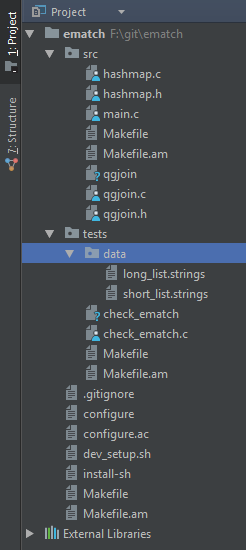
\includegraphics[width=0.5\textwidth]{folder_struct}
\end{figure}

Auf programmatischer Ebene wurde das Programm in zwei Abschnitte unterteilt:
\begin{itemize}
    \item \textbf{Vorbereitung} \\
    Hier werden Daten aus der ersten Datei geladen und benötigte Datenstrukturen im Speicher angefordert.
    Variablen werden initialisiert und der QGram Pool erstellt.
    \item \textbf{Ausführung} \\
    Das zweite Set an Daten wird über einen File Pointer referenziert und die
    Strings werden Zeile für Zeile ausgelesen, ihre QGramme mit denen im Schritt
    Vorbereitung erstellten verglichen und bei einer genügenden Übereinstimmung
    über STDOUT ausgegeben.
\end{itemize}

Hieraus ergaben sich 8 Sub-komponenten, welche einer Implementierung bedurften:


\begin{itemize}
    \item \textbf{Vorbereitung}:
    \begin{itemize}
        \item \textbf{S}: Eine Menge aller Strings aus der ersten Liste bzw Datei
        \item \textbf{Q}: Eine Menge aller QGramme, welche sich aus denjeweils einzelnen Strings in S generieren lassen
    \end{itemize}

    \item Ausführung
    \begin{itemize}
        \item \textbf{I}: Eine Menge, welche die gleiche Größe wie S ist und die
        Anzahl der Qgramme zählt, welche für den jeweiligen Index eines Strings in
        S passen.
        \item \textbf{f}: Eine Referenz zur zweiten Liste, von der wir zur vergleichende
        Strings holen können
        \item \textbf{T}: Eine Menge der Qgramme in der zur Zeit ausgelesenen Zeile
        \item \textbf{M}: Eine Menge der Indizes von Strings, welche auf die QGramme
        T am besten passen
    \end{itemize}
\end{itemize}

Mit Ausname von Q und M können alle Datenstrukturen mit den geläufigen C
Datentypen ausgedrückt werden.

Für die Strukturen Q und M mussten jedoch neue Datenstrukturen
erstellt werden. Für Q bot sich hier eine Hashmap an - prinzipiell besteht
hier zwar ein höherer Speicheraufwand, dieser ist jedoch abschätzbar, da die
maximale Anzahl an möglichen Key-Value Einträgen begrenzt ist. Der darausfolgende
O(1) Suchaufwand zum vergleich von Qgramme ist ein unschätzbarer Vorteil in der
späteren Ausführung. Auch hier wurde wiederum eine Nutzwertanalyse\ref{nwa_datentyp} durchgeführt,
um sicherzustellen dass die persönlichen Annahmen des Autors mit den technischen
Gegebenheiten übereinstimmen.
Hierzu wurden verschiedene Datenstrukturen nach folgenden Kriterien bewertet:

\begin{enumerate}
    \item \textbf{Speicheraufwand} \\
    Da laut Vorgabe maximal 32GB zur Ausführung des Programms zur Verfügung stehen,
    sollte der Speicherverbrauch natürlich so gering wie möglich sein. Da jedoch
    die maximale Datengröße aufgrund der 7-Bit ASCII Kodierung der Strings
    bekannt ist, ist dieses Kriterium am geringsten gewichtet worden.\par
    \item \textbf{Schnelligkeit Einfügen-Befehl} \\
    Das Erstellen der Datenstruktur sollte der größte rechnerische Aufwand im
    ersten Schritt des Programms sein. Deshalb sollte hier möglichst effizient gearbeitet und
    der Aufwand entsprechend optimiert sein.\par
    \item \textbf{Schnelligkeit Such-Befehl} \\
    Einen Wert aus der Datenstruktur abzufragen sollte nach möglichkeit in
    Richtung von Aufwand O(1) gehen, da dies mehrfach während des Stringvergleichs
    gebraucht wird. Deshalb ist dieses Kriterium auch am höchsten Gewichtet worden,
    da hier die größten Engpässe entstehen können.\par

\end{enumerate}

Für M wird eine dynamisch wachsende Array benötigt, da die Anzahl der passenden
QGramme je nach String variiert. Da die Anzahl der möglichen Zeichen pro QGramm von unserem
verwendeten Zeichensatz begrenzt ist (7-Bit ASCII), konnte eine begründete Annahme
über die Verteilung der QGramme in der Menge der Strings gemacht werden. Diese wurde anhand eines
Graphen\ref{qgram_verteilung} dargestellt. Die Verteilung stellt als Quantil die 
Menge an Qgrammen der String Daten dar.
Anhand dieser Analyse konnte eine optimale Startgröße festlegt werden, sodass in etwa der Hälfte der Fälle
erwartet werden kann, dass das Array nicht vergrößert werden muss, und somit die
Speicherzuweisungen minimiert werden.

\begin{figure}[!htp]
	\label{qgram_verteilung_klein}
	\caption{Qgramverteilung der Daten. Hochauflösung im Anhang.}
	\includegraphics[width=.25\textwidth]{multiplicity_of_qgrams}
\end{figure}

In Einklang mit der test-getriebenen Entwicklung wurde von Anfang an ein Hauptaugenmerk
auf die möglichst granulare Entwicklung des Codes gelegt. So wurden die Schritte
des Algorithmus in jweils mindestens einen Test und eine dazugehörige Funktion unterteilt \ref{listing_tests}.
Auch wurden für jeden selbsterstellten Datentypen und dazugehörige Funktionen
ebenfalls zunächst ein Test geschrieben.



\subsection{Entwurf der Benutzeroberfläche}
Der GNU Codingstandard\footnote{\url{https://www.gnu.org/prep/standards/standards.html\#User-Interfaces}},
sowie die POSIX Utility Guidelines\footnote{\url{http://pubs.opengroup.org/onlinepubs/9699919799/basedefs/V1_chap12.html}}
spezifizieren standardisierte Parameternamen und Funktionen eines Programms, sowie
deren erwartete Funktion. Da es sich bei der Zielgruppe um erfahrene Linuxnutzer handelt, wurde das
Kommandozeilenprogramm nach diesen Standards auch entwickelt. Ein Auszug dieser
Vorgaben befindet sich im Anhang auf Seite X.\par

Auf eine grafische Nutzeroberfläche wird nicht gewünscht, da die bevorzugte
Oberfläche der Endnutzer die Kommandozeile ist.

\subsection{Datenmodell}
Aufgrund der Natur der Daten ist das Datenmodell für das Projekt trivial. Es besteht aus einer
einspaltigen Tabelle, welche in Relation zu sich selbst steht. Ein Modell eines Strings sieht dann wie folgt aus:

aus diesen Gründen wird auf eine weitere Ausführung des Modells verzichtet.

Es ist zu klärifizieren, dass die GA Financial Solution kaum bis gar nicht Datenbanksysteme wie
MySQL, MariaDB u.Ä. nutzt. Stattdessen werden komprimmierte csv Dateien verwendet, welche
meist nur aus 3 Zeilen (Zeitstempel, Typ und Wert) bestehen. Dies ergibt sich aus
der negativen Erfahrung mit Datenbankmanagementsystemen und der Vereinfachung des Workflows durch
die Nutzung von CSV Daten in Kombination mit der hauseigenen CLI Toolchain.


\subsection{Geschäftslogik}
Die bisherige Geschäftslogik wird auf Seite X im Anhang dargestellt. Wie dort zu erkennen ist,
ist die Abholung der Daten von Anbietern automatisiert, die Verarbeitung jedoch nicht.
Diese geschieht bei Bedarf und erfordert u.A. die Vorsortierung der Daten in handhabbare
Datensätze, welche einfacher und in angemessener Zeit von unseren 4 Kern Maschinen
berechnet werden können. Zudem kommt noch eine erforderliche manuelle Überprüfung
der Ergebnisse. Die Darausentstehenden Daten werden schließlich für das derzeitig entwickelte Projekt
genutzt und schlussendlich wieder verworfen, da die Datensätze hoch parametrisiert sind,
und nicht zur generellen Nutzung innerhalb der Firma eignen.\par

Im Anhang auf Seite X ist ein Komponentendiagramm vorzufinden, welche die
unterschiedlichen Komponenten innerhalb der Geschäftslogik darstellt.

\subsection{Pflichtenheft / Datenverarbeitungskonzept}
Abschließend zur Entwurfsphase wurde ein Pflichtenheft erstellt und dieses als
Roter Faden für das Projekt der Abteilung für Datenverarbeitung vorgelegt. Wie im
Projektmanagement üblich, baut dieses auf dem Lastenheft auf.
Ein Auszug des Pflichtenhefts befindet sich im Anhang.

\clearpage

\label{section:implementierungsphase}
\section{Implementierungsphase}
\label{section:implementierungsphase}
\subsection{Entwicklungsvorbereitung}
Zunächst mussten einige organisatorische Bedingungen erfüllt werden, bevor die eigentliche Entwicklungsphase offiziell beginnen konnte. So wurden das Kanban Board mit den
Aufgabenpaketen aus dem Pflichtenheft populiert. Hierzu wurden Tests und deren
dazugehörigen Funktionen separat betrachtet und als Arbeitspaket beschrieben.

\subsection{Implementierung der Datenstruktur}
Wie bereits im vorherigen Abschnitt erwähnt, werden zwei spezielle Datenstrukturen für das Programm benötigt - Hashmaps und dynamisch wachsende Arrays.

\subsubsection{Hashmap-Implementierung}


Auf die eigene Implementierung einer Hashmap wurde verzichtet, stattdessen wurde
eine frei verfügbare Bibliothek genutzt, welche eine Hashmap für
String-Integer Paare zur Verfügung steht.

Der Code wurde weitgehend verbatim übernommen, mit der Ausnahme des
Containertyps, welche die Hashmap speichert. Da ein Q-Gramm in mehreren Strings
vorkommen kann, musste der Containertyp von einem Integer zu einen dynamisch
wachsenden Array abgewandelt werden. Da letzteres ohnehin entwickelt werden muss,
war die Komplexität dieser Anforderung gering.

\subsubsection{Dynamische Array-Implementierung}
C stellt nur simple Datentypen zur Verfügung, welche dem Nutzer erlauben komplexere Datenstrukturen abzubilden. Da ein dynamisch-wachsendes
Array nicht in C zur Verfügung steht, musste eine Datenstruktur für dieses erstellt werden.
Das Konzept hierbei ist recht einfach - sollte das Array voll sein, so wird beim
nächsten Aufruf der Insert-Funktion die Länge des Array verdoppelt. Hierfür wurde eine neue Datenstruktur angelegt und drei Funktionen definiert, um mit der Datenstruktur interagieren zu können. Ein Auszug des Quellcodes dieser Datenstruktur ist im Anhang zu finden \ref{lising:arrayImplementation}.\par

\clearpage
\clearpage

\label{section:abnahmephase}
\section{Abnahmephase}
Nach dem Abschluss der Implementationsphase wurde das Projekt, wie zuvor mit der
Abteilung für Datenverarbeitung vereinbart sowohl dem Abteilungsleiter im Einzelgespräch,
als auch der gesamten Abteilung in Form einer Präsentation vorgeführt.

Der Hauptaugenmerk und die Vorgehensweise war in beiden Fällen jedoch unterschiedlich
und wird in den folgenden Sektionen genauer erläutert.

\subsection{Code-Flight mit der Abteilungsleitung}

Um die Qualität des Codes zu gewährleisten wurde anstatt einer stillen Abnahme,
bei dem das Projekt übergeben, vom Auftraggeber überprüft und entweder abgenommen
oder bemängelt wird, wurde für das Projekt die Abnahme über einen
Code-Flight\footnote{zu deutsch "Programm-Flug"} festgelegt. Diese einstündige
Vorführung des Codes wurde mit dem Abteilungsleiter Sebastian Freundt im
Vier-Augen-Gespräch vollzogen und gestaltete sich wie folgt:

\begin{itemize}
    \item Demonstration des Programms über die Kommandozeile, mit Schritt-für-Schritt Erklärung der gewählten Parameter und deren Design-Entscheidung.
    \item Sichtung des Codes, angefangen mit der Hauptroutine.
    \item Erläuterung der gewählten Datenstrukturen und die Begründung für die Nutzung dieser.
    \item Limitation des Algorithmus und des CLI Programms.
    \item Die nächsten, möglichen Schritte zur Verbesserung der Hauptprogramms.
    \item Mögliche Ansätze zur Verbesserung des Algorithmus.
\end{itemize}

\subsection{Präsentation des Programms}

Nachdem der Code-Flight mit dem Abteilungsleiter abgeschlossen wurde, wurde ebenfalls
eine Präsentation für das gesamte Team der Abteilung Datenverarbeitung gehalten.
Diese beschränkte sich im Inhalt jedoch auf die Grundprinzipien des Algorithmus, sowie
die Funktion und Nutzung des CLI Programms. Unter anderem wurden verfügbare
Parameter und maximal-zulässige Dateigrößen erläutert.

\subsection{Zwischenstand}

\clearpage

\label{section:dokumentationsphase}
\section{Dokumentation}
\label{section:dokumentationsphase}
Die Dokumentation ist aufgeteilt in zwei Bestandteile: Die Nutzerdokumentation
in Form einer CLI-Dokumentation, sowie die Entwicklerdokumentation in Form von
Dokumentationsblöcken im Quellcode. Die gesamte Dokumentation wurde auf Englisch,
der Sprache des Unternehmens, verfasst.

\subsection{Nutzerdokumentation}
Da der Funktionsumfang des Programms recht klein ist, wird auf ein handelsübliches
Dokument verzichtet. Die Dokumentation findet ausschließlich über die Kommandozeile mit dem Aufruf des Programms unter Zusatz des Hilfe-Parameters (''help'' bzw. ''h'') statt.
Dieser Aufruf erzeugt eine kurze Beschreibung des Programms und dessen Parameter.

\subsection{Entwicklerdokumentation}
Die Entwicklerdokumentation des Codes findet über einen
Dokumentationsblock oberhalb der Signatur jeder Funktion statt. Dieser Block
beinhaltet eine kurze Beschreibung der Funktionsweise der Routine sowie die
Namen und erwarteten Datentypen der Funktionsparameter. Die Formatierung ist
ReStructuredText (kurz ReST), kann mit Hilfe von Dokumentationstools ausgelesen
und später als eine lokale Webseite mit automatisch generierten Verlinkungen ausgegeben werden.

\clearpage

\section{Fazit}
\label{section:postmortem}
\subsection{Soll- /Ist-Vergleich}
Rückblickend kann festgehalten werden, dass alle, im Pflichtenheft
abgesprochenen Funktionen und Anforderungen eingehalten worden sind,
und zur vollsten Zufriedenheit des Auftraggebers erstellt wurden. Hierbei
spielt die Entscheidung, die Einbindung des C Codes in Python zu streichen, sicherlich
eine elementare Rolle. Wie man erkennen kann, wurden die Stunden, welche durch
die Streichung frei wurden, effektive und vollsten ausgenutzt um den Anforderungen
des Projekts gerecht zu werden. Dabei wurden die von der IHK vorgegebenen 70 Stunden
konsequent eingehalten.

\subsection{Post Mortem}

Vor Allem die Entwurfsphase half dem Autor seine Kenntnisse aus dem Projektmanagement anzuwenden,
und waren bei den Nutzwertanalysen besonders hilfreich. Auch erwies sich die Anwendung des
testgetriebenen Entwicklungskreislaufs als große Unterstützung dar - so wurden lästige Segmentation Faults frühzeitig
erkannt, und die Funktionen (und somit das gesamt Programm) konnten schneller zu produktionsreife heranwachsen.
Auch das genutzte Kanban-Board erwies sich als großartiges Werkzeug, um Prozesse und deren Fortschritt zu dokumentieren.
Kurze Kommunikations- und Entscheidungswege ermöglichten eine agile Entwicklung der Projekts und werden
dem Autor auch weiterhin als ein wichtiger Baustein produktiver Arbeitsumgebungen in Erinnerung bleiben.

\subsection{Ausblick}
Punkte, welche im Lastenheft genannt, aber nicht mit in das Pflichtenheft genommen worden,
stehen nun natürlich auf der Liste der weiteren Schritte. Da der Code gut dokumentiert
und mit viel Auge für Lesbarkeit geschrieben worden ist, ist eine Cythoneinbindung nun effizient umsetzbar.
Durch die bereitgestellten Tests können ebenfalls schnell Python Unittests erstellt, und somit
die Einbindung des C Codes effektiv und verlässlich auch in Python überprüft werden.

Schlussendlich bleiben noch zwei Punkte, welche in Zukunft angegangen werden könnten, um das Programm weiter zu verfeinern:
\begin{enumerate}

\item Die Optimierung der Programmlogik \\
    \begin{itemize}
        \item Verfeinerung der Hashmap - Da die maximale Anzahl an Schlüsselwörten bekannt ist, kann die Hashmap so implementiert werden, dass exakt so viele ''Felder'' im Speicher reserviert werden wie nötig - und kein einziges mehr.
        \item Das Auswahlkriterium könnte als Funktion implementiert, und der Vergleichsfunktion als Pointer übergeben werden. So könnten Änderungen noch unkomplizierter realisiert werden.
    \end{itemize}


\item Weiteres fine-tuning des Q-Gramm Filters


\end{enumerate}




\clearpage

\section{Anhang}
\subsection{Analysephase}
\subsubsection{Vergleich: DLD Aufwand vs QGram Aufwand mit Fuzzy Join}
\subsubsection{Vergleich: Theoretischer DLD vs QGram Zeitvergleich }
\subsubsection{Projektkosten}
\begin{table}[!htp]
	\centering
	\caption{Projektkosten}
	\label{tabelle:projektkosten}
	\begin{tabular}{llllll}
		\rowcolor[HTML]{9698ED}
		{\color[HTML]{FFFFFF} \textbf{Vorgang}} & {\color[HTML]{FFFFFF} \textbf{Mitarbeiter}} & {\color[HTML]{FFFFFF} \textbf{Stunden}} & {\color[HTML]{FFFFFF} \textbf{Personal}} & {\color[HTML]{FFFFFF} \textbf{Ressources}} & {\color[HTML]{FFFFFF} \textbf{Gesamt}} \\
		Entwicklungskosten                      & 1                                           & 70                                      & 385.00 €                                 & 1,295.00 €                                 & 1,680.00 €                             \\
		\rowcolor[HTML]{BBDAFF}
		Fachgespräch                            & 2                                           & 5                                       & 350.00 €                                 & 92.50 €                                    & 1,842.50 €                             \\
		Code Review                             & 2                                           & 2                                       & 140.00 €                                 & 37.00 €                                    & 317.00 €                               \\
		\rowcolor[HTML]{BBDAFF}
		Abnahme                                 & 2                                           & 0.5                                     & 35.00 €                                  & 9.25 €                                     & 44.25 €                                \\
		&                                             &                                         & \multicolumn{2}{l}{\textbf{Projektkosten Gesamt:}}                                    & \textbf{3,883.75 €}
	\end{tabular}
\end{table}

\subsubsection{Lastenheft}
\renewcommand{\labelenumii}{\theenumii}
\renewcommand{\theenumii}{\theenumi.\arabic{enumii}.}
\begin{enumerate}
    \item Spezifikationen des Algorithmus
        \begin{enumerate}
            \item Der Algorithmus muss 2 Listen von Strings verarbeiten können,
            wobei eine dieser Listen garantiert in den Speicher passt und die zweite
            eine beliebige Größe haben kann.
            \item Der Algorithmus muss aus der ersten Liste sämtliche Strings finden,
            welche den Strings aus der zweiten Liste ähneln. Die gefundenen Strings
            sollen ausgegeben werden.
            \item Der Algorithmus ist in C zu programmieren.
            \item der Algorithmus verarbeitet 7-Bit ASCII Strings schreibungsunabhängig. Zeichensetzung
            ist beim Vergleich generell zu ignorieren; Ausnahmen bilden die
            Charaktere Bindestrich, Unterstrich und Leerzeichen.
        \end{enumerate}
    \item Spezifikationen des Kommandozeilenprogramms
        \begin{enumerate}
            \item Der Algorithmus muss über die Kommmandozeile ausführbar sein.
            \item Die Erste Liste wird immer als Dateiname übergeben.
            \item Die zweite Liste kann entweder als Dateiname oder über STDIN übergeben werden.
            \item die GNU Standards für Kommandozeilenprogramme müssen eingehalten werden.
            \item Die POSIX Utility Guidelines müssen eingehalten werden.
            \item Das Programm muss unter openSuSE 13.1 laufen.
            \item Alle für das Programm erforderliche Abhängigkeiten
            (z.B. Pakete, Bibliotheken) müssen für openSuSE 13.1 verfügbar sein.
            \item Das Programm muss auf einem einzigen Kern lauffähig sein, und
            darf das laufen auf mehreren Kernen in einem Shared-Memory-Environment
            unterstützen.
            \item Das Programm darf mit maximal 32GB Arbeitsspeicher arbeiten, und nicht mehr
            als 200 GB Festplattenspeicher zur Kalkulation verwenden. Zwischenprozessliche Kommunikationswege
            sind ausgeschlossen.
            \item Das Programm gibt Fehler und Debug Daten über STDERR aus.
            \item Errechnete Ergebnisse werden über STDOUT ausgegeben.
            \item Die Zielplatform ist Intel x86-64 (intel64).
        \end{enumerate}
    \item Spezifikationen der Qualitätssicherung
        \begin{enumerate}
            \item Der Algorithmus muss überprüfbar sein.
            \item Unittests sind verfügbar gemacht worden.
        \end{enumerate}
    \item Spezifikationen der Dokumentation
        \begin{enumerate}
            \item Sämtliche Funktionen müssen über einen Doc String dokumentiert werden
            \item Die Doc Strings der Funktionen müssen auf Englisch geschrieben werden.
        \end{enumerate}
\end{enumerate}

\subsubsection{Nutzwertanalyse: Projektentwicklung}
\begin{table}[!htp]
	\centering
	\caption{Nutzwertanalyse Projektentwicklung}
	\label{nwa:projektentwicklung}
	\begin{tabular}{llllllllll}
		\rowcolor[HTML]{9698ED}
		{\color[HTML]{FFFFFF} \textbf{Kriterien}} & {\color[HTML]{FFFFFF} \textbf{Gewicht}} & {\color[HTML]{FFFFFF} \textbf{Externe Entwicklung}} & {\color[HTML]{FFFFFF} \textbf{}}       & {\color[HTML]{FFFFFF} \textbf{Interne Entwicklung}} & {\color[HTML]{FFFFFF} \textbf{}}       & {\color[HTML]{FFFFFF} \textbf{Dedizierter 12-Kerner}} & {\color[HTML]{FFFFFF} \textbf{}}       & {\color[HTML]{FFFFFF} \textbf{Cluster}}   & {\color[HTML]{FFFFFF} \textbf{}}       \\
		\rowcolor[HTML]{9698ED}
		{\color[HTML]{FFFFFF} \textbf{}}          & {\color[HTML]{FFFFFF} \textbf{}}        & {\color[HTML]{FFFFFF} \textbf{Bewertung}}           & {\color[HTML]{FFFFFF} \textbf{Gesamt}} & {\color[HTML]{FFFFFF} \textbf{Bewertung}}           & {\color[HTML]{FFFFFF} \textbf{Gesamt}} & {\color[HTML]{FFFFFF} \textbf{Bewertung}}             & {\color[HTML]{FFFFFF} \textbf{Gesamt}} & {\color[HTML]{FFFFFF} \textbf{Bewertung}} & {\color[HTML]{FFFFFF} \textbf{Gesamt}} \\
		Projektkosten                             & 45.00\%                                 & 4                                                   & 1.8                                    & 5                                                   & 2.25                                   & 4                                                     & 1.8                                    & 3                                         & 1.35                                   \\
		\rowcolor[HTML]{BBDAFF}
		Nachhaltigkeit                            & 15.00\%                                 & 4                                                   & 0.6                                    & 4                                                   & 0.6                                    & 1                                                     & 0.15                                   & 1                                         & 0.15                                   \\
		Flexibilit채t                              & 5.00\%                                  & 3                                                   & 0.15                                   & 5                                                   & 0.25                                   & 4                                                     & 0.2                                    & 4                                         & 0.2                                    \\
		\rowcolor[HTML]{BBDAFF}
		Unterhaltskosten                          & 35.00\%                                 & 4                                                   & 1.4                                    & 4                                                   & 1.4                                    & 2                                                     & 0.7                                    & 1                                         & 0.35                                   \\
		\textbf{Gesamt}                           & \textbf{100.00\%}                       & \textbf{}                                           & \textbf{3.95}                          & \textbf{}                                           & \textbf{4.5}                           & \textbf{}                                             & \textbf{2.85}                          & \textbf{}                                 & \textbf{2.05}
	\end{tabular}
\end{table}

\subsubsection{Use-Case QGJoin}

\subsection{Entwurfsphase}
\subsubsection{Nutzwertanalyse: Programmiersprachen}

\begin{table}[!htp]
    \centering
    \caption{Nutzwertanalyse der Programmiersprachen}
    \label{nwa:sprachen}
    \begin{tabular}{llllllllll}
        \rowcolor[HTML]{9698ED}
        {\color[HTML]{FFFFFF} \textbf{Kriterien}} & \multicolumn{1}{c}{\cellcolor[HTML]{9698ED}{\color[HTML]{FFFFFF} \textbf{Gewicht}}} & \multicolumn{2}{c}{\cellcolor[HTML]{9698ED}{\color[HTML]{FFFFFF} \textbf{C}}}                                                                                              & \multicolumn{2}{c}{\cellcolor[HTML]{9698ED}{\color[HTML]{FFFFFF} \textbf{C++}}}                                                                                            & \multicolumn{2}{c}{\cellcolor[HTML]{9698ED}{\color[HTML]{FFFFFF} \textbf{Java}}}                                                                                           & \multicolumn{2}{c}{\cellcolor[HTML]{9698ED}{\color[HTML]{FFFFFF} \textbf{Haskell}}}                                                                                        \\
        \rowcolor[HTML]{9698ED}
        {\color[HTML]{FFFFFF} \textbf{}}          & \multicolumn{1}{c}{\cellcolor[HTML]{9698ED}{\color[HTML]{FFFFFF} \textbf{}}}        & \multicolumn{1}{c}{\cellcolor[HTML]{9698ED}{\color[HTML]{FFFFFF} \textbf{Bewertung}}} & \multicolumn{1}{c}{\cellcolor[HTML]{9698ED}{\color[HTML]{FFFFFF} \textbf{Gesamt}}} & \multicolumn{1}{c}{\cellcolor[HTML]{9698ED}{\color[HTML]{FFFFFF} \textbf{Bewertung}}} & \multicolumn{1}{c}{\cellcolor[HTML]{9698ED}{\color[HTML]{FFFFFF} \textbf{Gesamt}}} & \multicolumn{1}{c}{\cellcolor[HTML]{9698ED}{\color[HTML]{FFFFFF} \textbf{Bewertung}}} & \multicolumn{1}{c}{\cellcolor[HTML]{9698ED}{\color[HTML]{FFFFFF} \textbf{Gesamt}}} & \multicolumn{1}{c}{\cellcolor[HTML]{9698ED}{\color[HTML]{FFFFFF} \textbf{Bewertung}}} & \multicolumn{1}{c}{\cellcolor[HTML]{9698ED}{\color[HTML]{FFFFFF} \textbf{Gesamt}}} \\
        Performanz                                & 30.00\%                                                                             & 5                                                                                     & 1.5                                                                                & 5                                                                                     & 1.5                                                                                & 4                                                                                     & 1.2                                                                                & 5                                                                                     & 1.5                                                                                \\
        \rowcolor[HTML]{BBDAFF}
        Speichereffizienz                         & 30.00\%                                                                             & 5                                                                                     & 1.5                                                                                & 5                                                                                     & 1.5                                                                                & 3                                                                                     & 0.9                                                                                & 4                                                                                     & 1.2                                                                                \\
        Dokumentation                             & 20.00\%                                                                             & 5                                                                                     & 1                                                                                  & 4                                                                                     & 0.8                                                                                & 4                                                                                     & 0.8                                                                                & 2                                                                                     & 0.4                                                                                \\
        \rowcolor[HTML]{BBDAFF}
        Systemische Vorraussetzungen              & 10.00\%                                                                             & 5                                                                                     & 0.5                                                                                & 5                                                                                     & 0.5                                                                                & 3                                                                                     & 0.3                                                                                & 3                                                                                     & 0.3                                                                                \\
        Datenstrukturen                           & 10.00\%                                                                             & 3                                                                                     & 0.3                                                                                & 4                                                                                     & 0.4                                                                                & 5                                                                                     & 0.5                                                                                & 5                                                                                     & 0.5                                                                                \\
        \rowcolor[HTML]{BBDAFF}
        \textbf{Gesamt}                           & \textbf{100.00\%}                                                                   & \textbf{}                                                                             & \textbf{4.8}                                                                       & \textbf{}                                                                             & \textbf{4.7}                                                                       & \textbf{}                                                                             & \textbf{3.7}                                                                       & \textbf{}                                                                             & \textbf{3.9}
    \end{tabular}
\end{table}

\subsubsection{Nutzwertanalyse: Datentyp der Menge Q}

\begin{table}[!htp]
    \centering
	\caption{Nutzwertanalyse der Datentypen für Q}
    \label{nwa:datentyp}
    \begin{tabular}{llllll}
        \rowcolor[HTML]{9698ED}
        \cellcolor[HTML]{9698ED}{\color[HTML]{FFFFFF} }                                     & \cellcolor[HTML]{9698ED}{\color[HTML]{FFFFFF} }                                   & \multicolumn{2}{l}{\cellcolor[HTML]{9698ED}{\color[HTML]{FFFFFF} \textbf{Hashmap}}} & \multicolumn{2}{l}{\cellcolor[HTML]{9698ED}{\color[HTML]{FFFFFF} \textbf{Binärbaum}}} \\
        \rowcolor[HTML]{9698ED}
        \multirow{-2}{*}{\cellcolor[HTML]{9698ED}{\color[HTML]{FFFFFF} \textbf{Kriterien}}} & \multirow{-2}{*}{\cellcolor[HTML]{9698ED}{\color[HTML]{FFFFFF} \textbf{Gewicht}}} & {\color[HTML]{FFFFFF} \textbf{Bewertung}}  & {\color[HTML]{FFFFFF} \textbf{Gesamt}} & {\color[HTML]{FFFFFF} \textbf{Bewertung}}   & {\color[HTML]{FFFFFF} \textbf{Gesamt}}  \\
        Speicheraufwand                                                                     & 25.00\%                                                                           & 2                                          & 0.5                                    & 2                                           & 0.5                                     \\
        \rowcolor[HTML]{BBDAFF}
        Schnelligkeit Daten Einfügen (Insert                                                & 20.00\%                                                                           & 5                                          & 1                                      & 4                                           & 0.8                                     \\
        Schnelligkeit Auslesen (Look-up)                                                    & 55.00\%                                                                           & 5                                          & 2.75                                   & 4                                           & 2.2                                     \\
        \rowcolor[HTML]{BBDAFF}
        \textbf{Gesamt}                                                                     & \textbf{100.00\%}                                                                 & \textbf{}                                  & \textbf{4.25}                          & \textbf{}                                   & \textbf{3.5}
    \end{tabular}
\end{table}

\subsubsection{Pseudocode: Algorithmus}
\subsubsection{Aktivitätsdiagramm: Programmlogik}
\begin{figure}[!htp]
    \caption{Aktivitätsdiagramm der Programmlogik}
    \label{programmlogik}
    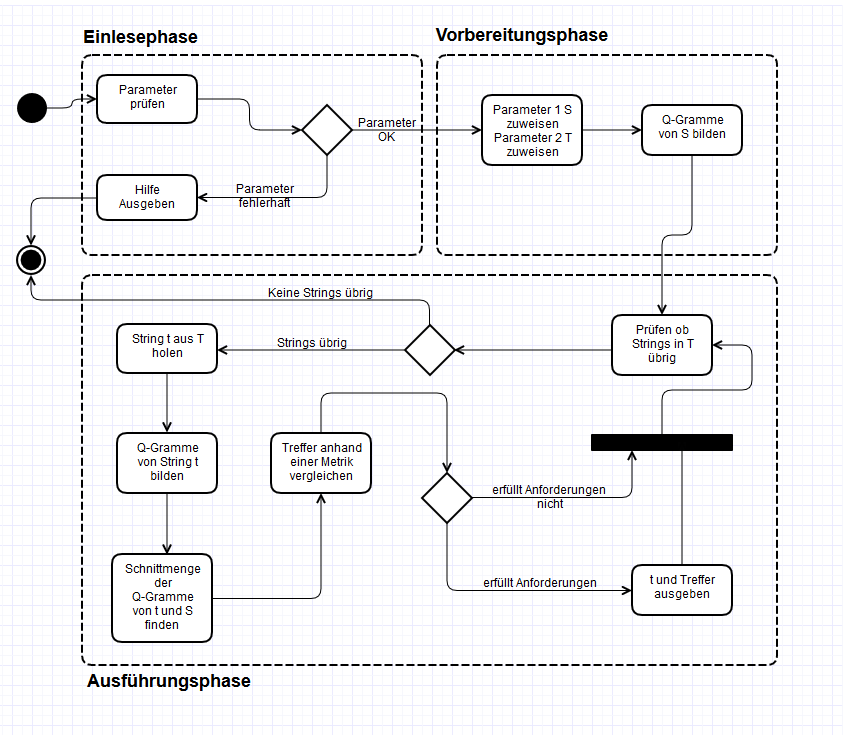
\includegraphics[width=\textwidth]{algo}
    \centering
\end{figure}

\subsubsection{Analyse: Verteilung der Qgramme}
\begin{figure}[!htp]
    \caption{Verteilung der QGramme im zu bearbeitenden Datensatz}
    \label{fig:qgram_verteilung}
    \includegraphics[width=\textwidth]{multiplicity_of_qgrams.eps}
    \centering
\end{figure}

\subsubsection{Datenmodell}
\begin{figure}[!htp]
    \caption{UML Darstellung des Datenmodells}
    \label{fig:datenmodell}
    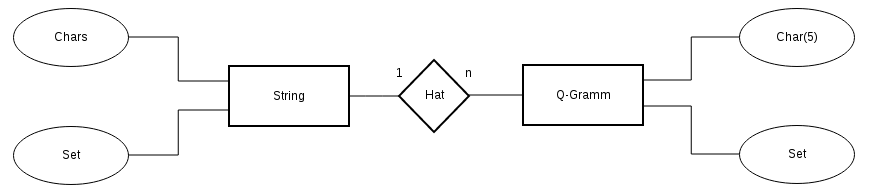
\includegraphics[width=\textwidth]{datenmodell}
    \centering
\end{figure}

\subsubsection{Pflichtenheft}

\subsection{Implementierungsphase}
\subsubsection{Quellcodeauszug: Dynamische Array}
\lstinputlisting[language=C, label=lising:arrayImplementation, caption=Auszug aus dem C Quellcode der dynamischen Array]{anhang/array.c}

\subsubsection{Quellcodeauszug: Hashtable Implementation}
\lstinputlisting[language=C, label=listing:hashtableImplmentation, caption=Auszug aus dem C Quellcode der dynamischen Array]{anhang/hashmap.c}

\subsubsection{Auszug: Hilfeausgabe des Kommandozeilenprogramms}

\subsection{Dokumentationsphase}
\subsubsection{Auszug: Entwicklerdokumentation}
\lstinputlisting[language=C, label=listing:entwicklerDoku, caption=Beispiel eines Docstrings für Entwickler]{anhang/docstring.c}

\subsubsection{Auszug: Endnutzerdokumentation}


\bibliography{bibliography}
%---------------------------------------------------------------------------
\end{document}
%---------------------------------------------------------------------------
